\subsection{Modelo de operaciones}

\subsubsection{Diagrama de casos de uso}

En este primer modelo mostraremos todos los escenarios en los que algún agente (encargados, clientes, locales, gerente, etc) participa en alguna operación del sistema. A estos agentes los llamaremos actores y los representamos con la figura de una persona. También mostraremos las relaciones de extensión e inclusión entre las operaciones, en caso de que existan. Luego, detallaremos por completo los pasos que conlleva realizar cada una de las operaciones, es decir, como el actor (o actores) que participan en dicha operación interactúan con nuestro sistema. También se visualizan relaciones de herencia entre actores, donde los casos de uso del actor padre también pertenecen al actor hijo.

Si bien esta técnica detalla los pasos de una operación y muestra los actores que participan en cada una, no permite visualizar un orden a seguir entre operaciones ni tampoco modelar aspectos puros del sistema (comportamiento automático en donde no hay actores). El orden entre operaciones lo mostraremos más adelante, cuando utilicemos diagramas de actividad.

A continuación mostraremos el diagrama de casos de uso resultante y el detalle de las operaciones de cada uno de los casos:

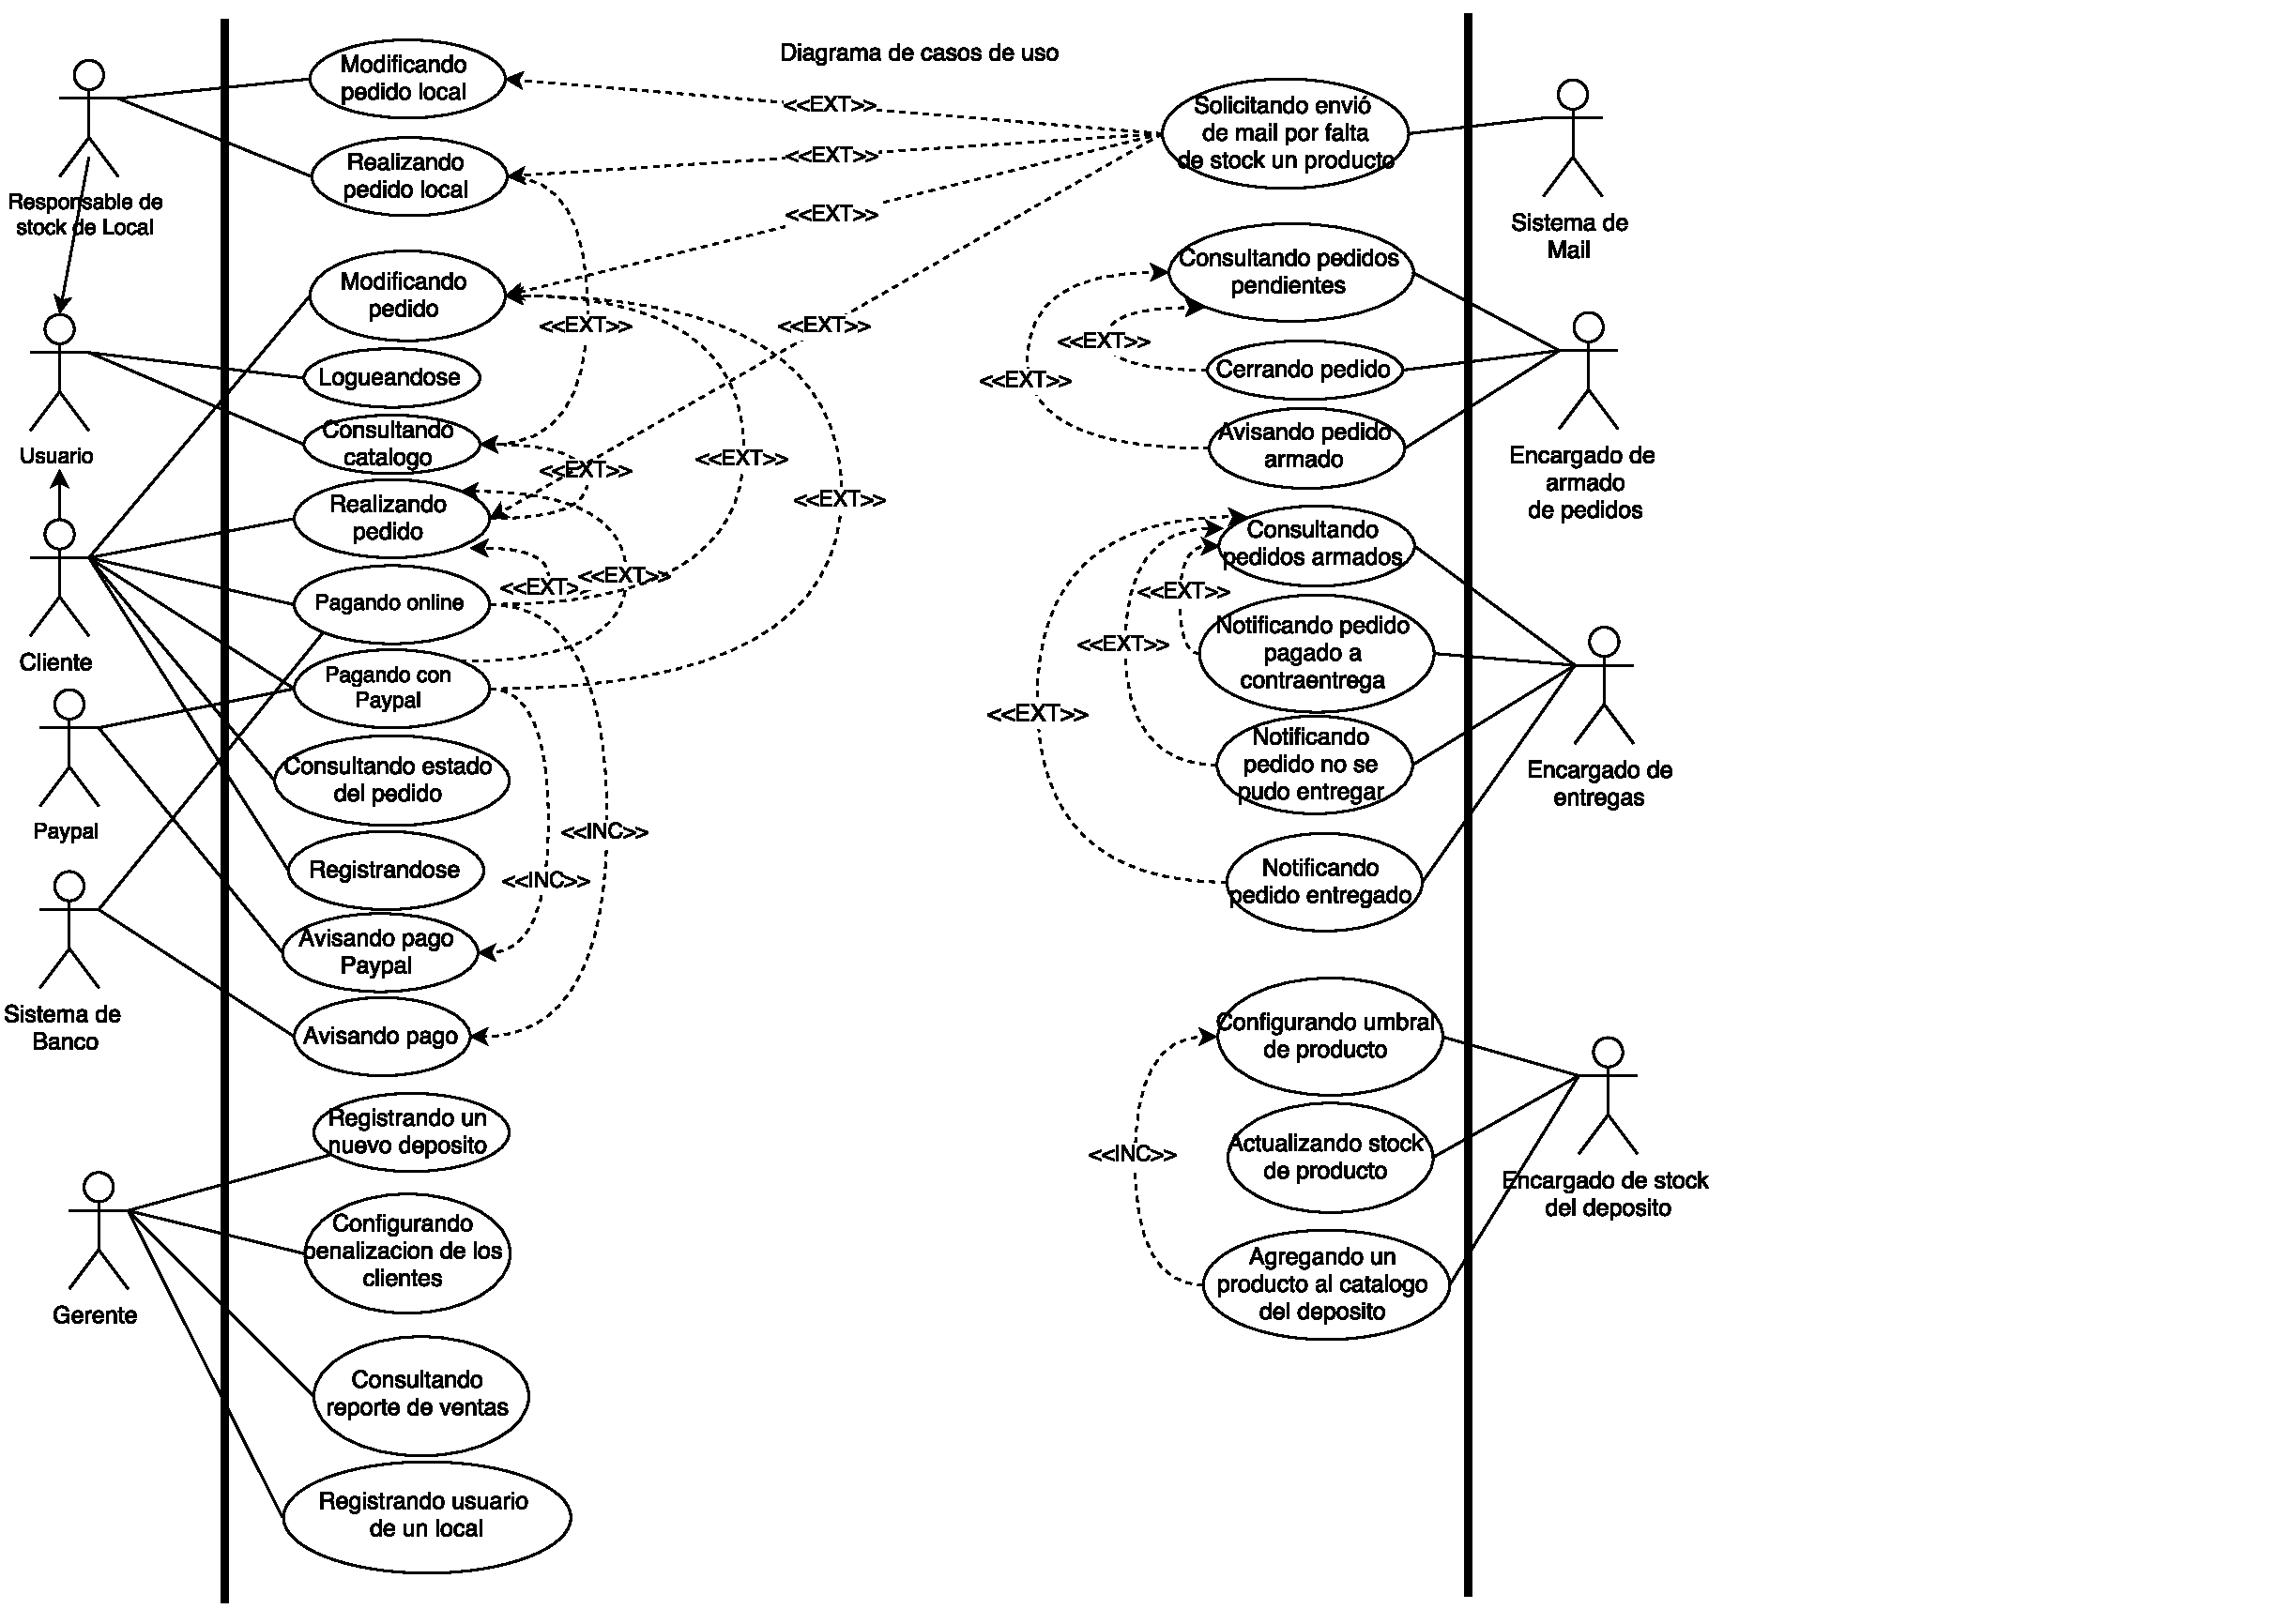
\includegraphics[scale=0.5, angle=90]{secciones/diagramaCasosUso}

\subsubsection{Detalle de los casos de uso}

\begin{tabular}{p{0.2\textwidth} p{0.8\textwidth}}
    \textsc{Caso de uso} & Registrándose \\
    \textsc{Actores} & Cliente \\
    \textsc{Pre} & - \\
    \textsc{Post} & El cliente se registra en el sitio \\
\end{tabular}

\begin{center}
\begin{tabular}{|p{0.4\textwidth}|p{0.4\textwidth}|}
    \hline
    \multicolumn{1}{|c|}{Curso Normal} &
    \multicolumn{1}{|c|}{Curso alternativo} \\
    \hline
    1. El cliente ingresa sus datos personales (nombre, apellido, DNI, domicilio y numero teléfono). & \\
    2. El cliente ingresa un nombre de usuario. & \\
    3. El cliente ingresa una contraseña. & \\
    4. El cliente sube al sitio una copia de su DNI. & \\
    5. El sistema valida que los datos ingresados no pertenezcan a un usuario
    existente. &
    5.1 Si los datos ya existen, volver al paso 1.  \\
    6. El sistema guarda los datos del usuario. & \\
    7. FIN CU. & \\
    \hline
\end{tabular}
\end{center}

\begin{tabular}{p{0.2\textwidth} p{0.8\textwidth}}
    \textsc{Caso de uso} & Logueandose \\
    \textsc{Actores} & Usuario \\
    \textsc{Pre} & El usuario debe estar registrado. \\
    \textsc{Post} & El usuario ingresa al sitio con su cuenta. \\
\end{tabular}

\begin{center}
\begin{tabular}{|p{0.4\textwidth}|p{0.4\textwidth}|}
    \hline
    \multicolumn{1}{|c|}{Curso Normal} &
    \multicolumn{1}{|c|}{Curso alternativo} \\
    \hline
    1. El usuario ingresa el nombre de su cuenta y su contraseña. & \\
    2. El sistema valida los datos. &
    2.1. Si los datos son incorrectos, volver al paso 1. \\
    3. FIN CU. & \\
    \hline
\end{tabular}
\end{center}

\begin{tabular}{p{0.2\textwidth} p{0.8\textwidth}}
    \textsc{Caso de uso} & Consultando catálogo. \\
    \textsc{Actores} & Usuario \\
    \textsc{Pre} & El usuario está logueado. \\
    \textsc{Post} & El usuario visualiza el catálogo de todos los productos
    disponibles. \\
\end{tabular}

\begin{center}
\begin{tabular}{|p{0.4\textwidth}|p{0.4\textwidth}|}
    \hline
    \multicolumn{1}{|c|}{Curso Normal} &
    \multicolumn{1}{|c|}{Curso alternativo} \\
    \hline
    1. El sistema muestra al usuario todos los productos disponibles en alguno de los depósitos del sistema y el stock disponible de cada uno en dicho depósito. & \\
    2. Si el usuario quiere realizar un pedido de productos. EXT CU:
    ``Realizando Pedido''. & \\
    3. FIN CU. & \\
    \hline
\end{tabular}
\end{center}

\begin{tabular}{p{0.2\textwidth} p{0.8\textwidth}}
    \textsc{Caso de uso} & Realizando pedido local. \\
    \textsc{Actores} & Responsable de stock del local \\
    \textsc{Pre} & El responsable de stock del local debe estar logueado y debe
    haber consultado el catálogo de productos previamente. \\
    \textsc{Post} & El responsable de stock del local realizó un pedido con
    éxito. \\
\end{tabular}

\begin{center}
\begin{tabular}{|p{0.4\textwidth}|p{0.4\textwidth}|}
    \hline
    \multicolumn{1}{|c|}{Curso Normal} &
    \multicolumn{1}{|c|}{Curso alternativo} \\
    \hline
    1. El sistema verifica que el responsable de stock del local no tenga un pedido pendiente de entrega. &
    1.1. Si el responsable de stock del local tiene un pedido pendiente, rechazar pedido. FIN CU. \\
    2. El responsable de stock del local selecciona el producto que desea
    adquirir. & \\
    3. El responsable de stock ingresa la cantidad de unidades que desea del
    producto. & \\
    4. El responsable de stock vuelve al paso 2 por cada producto que desea
    adquirir. & \\
    5. El responsable de stock confirma el pedido. & \\
    6. El sistema chequea que en el depósito haya suficiente stock disponible para cada producto solicitado en el pedido. &
    6.1. Si el stock disponible no es suficiente para alguno de los productos, mostrar al usuario un mensaje de error diciendo ``Stock insuficiente''. FIN CU. \\
    7. El sistema propone al responsable de stock tres posibles fechas al azar, en días hábiles, dentro de los próximos siete días para que le sea entregado su pedido. & \\
    8. El responsable de stock selecciona la fecha que desea en que le entreguen el pedido. & \\
    9. El sistema almacena los datos del pedido. & \\
	10. El sistema reserva en el depósito, por cada producto pedido, la cantidad solicitada de dicho producto. & \\
	11. Si el pedido causo que el stock de un producto sea menor que el umbral configurado para dicho producto, EXT CU: ``Solicitando envió de mail por falta de stock un producto''. & \\
	12. El sistema vuelve al paso 11 por cada producto que haya caído debajo de su umbral por causa de los productos pedidos. & \\
    13. FIN CU. & \\
    \hline
\end{tabular}
\end{center}

Es importante notar que el sistema solo arregla una fecha de entrega con el encargado de stock del local y no un horario. Es el encargado de entregas quien se encarga de entregar los pedidos a los locales en el horario en que estos operan.

\newpage

\begin{tabular}{p{0.2\textwidth} p{0.8\textwidth}}
    \textsc{Caso de uso} & Realizando Pedido. \\
    \textsc{Actores} & Cliente \\
    \textsc{Pre} & El Cliente está logueado y consultó el catálogo de
    productos. \\
    \textsc{Post} & El cliente realizó un pedido con éxito. \\
\end{tabular}


\begin{center}
\begin{tabular}{|p{0.4\textwidth}|p{0.4\textwidth}|}
    \hline
    \multicolumn{1}{|c|}{Curso Normal} &
    \multicolumn{1}{|c|}{Curso alternativo} \\
    \hline
    1. El sistema verifica que el cliente no esté penalizado. &
    1.1 Si el Cliente está penalizado, rechazar pedido. FIN CU. \\
    2. El sistema verifica que el cliente no tenga un pedido pendiente de entrega. &
    2.2 Si el Cliente tiene un pedido pendiente, rechazar pedido. FIN CU. \\
    3. El Cliente selecciona el producto que desea adquirir. & \\
    4. El Cliente ingresa la cantidad de unidades que desea del producto, la cual debe estar entre $1$ y el stock disponible en el depósito en ese momento. & \\
    5. El Cliente vuelve al paso 3 por cada producto que desea adquirir. & \\
    6. El sitio calcula el importe total del pedido. & \\
    7. El Cliente confirma el pedido. & \\
    8. El sistema chequea que en el depósito haya suficiente stock disponible para cada producto solicitado en el pedido. &
    8.1. Si el stock disponible no es suficiente para alguno de los productos, mostrar al cliente un mensaje de error diciendo ``Stock insuficiente''. FIN CU. \\
    9. El sistema propone al cliente tres posibles fechas al azar, en días hábiles, dentro de los próximos siete días para que le sea entregado su pedido. & \\
    10. El Cliente selecciona la fecha que desea en que le entreguen el pedido. & \\
    11. El Cliente selecciona el método de pago que desea entre Paypal, pagar con tarjeta de crédito o débito, o pagar a contraentrega. & \\
    12. Si el Cliente desea pagar con tarjeta de crédito o débito. EXT CU:
    ``Pagando Online''. & \\
    13. Si el Cliente desea pagar con PayPal. EXT CU: ``Pagando con PayPal''. & \\
    14. El sistema almacena los datos del pedido. & \\
    15. El sistema reserva en el depósito, por cada producto pedido, la cantidad solicitada de dicho producto. & \\
\end{tabular}
\end{center}

\begin{center}
\begin{tabular}{|p{0.4\textwidth}|p{0.4\textwidth}|}
    16. Si el pedido causo que el stock de un producto sea menor que el umbral configurado para dicho producto, EXT CU: ``Solicitando envió de mail por falta de stock un producto''. & \\
	17. El sistema vuelve al paso 16 por cada producto que haya caído debajo de su umbral por causa de los productos pedidos. & \\
    18. FIN CU. & \\
    \hline
\end{tabular}
\end{center}


Es importante notar que la cantidad de unidades de un producto que el cliente puede pedir es igual a la cantidad de unidades disponibles en el deposito en el momento que el cliente \textbf{inicia} el pedido. Esta cantidad pudo haber disminuido \textit{(por un pedido de otro usuario)} e impedir que el cliente concrete su pedido. En este caso, el cliente deberá iniciar la operación nuevamente.


Se verifica si el cliente está penalizado comprobando que haya una instancia de ``\textit{Penalización}'' asociada a la cuenta cuyo intervalo de fechas contenga a la fecha actual.
Se puede ver en más detalle el flujo de penalización en el modelo de máquinas de estado.


También existe un diagrama de actividad que muestra el orden completo del flujo de la realización de un pedido \textit{(por parte de un cliente)}, desde que se consulta el catálogo hasta que el pedido es entregado.

\vspace{2cm}

\begin{tabular}{p{0.2\textwidth} p{0.8\textwidth}}
    \textsc{Caso de uso} & Pagando Online. \\
    \textsc{Actores} & Cliente, Sistema de Banco \\
    \textsc{Pre} & El cliente está logueado y debe estar realizando un pedido. \\
    \textsc{Post} & El cliente realiza el pago del pedido vía online. \\
\end{tabular}

\begin{center}
\begin{tabular}{|p{0.4\textwidth}|p{0.4\textwidth}|}
    \hline
    \multicolumn{1}{|c|}{Curso Normal} &
    \multicolumn{1}{|c|}{Curso alternativo} \\
    \hline
    1. El cliente completa los datos de la tarjeta (tipo, nombre del titular,
    número, código de seguridad, fecha de vencimiento) &
    1.1 El usuario dejó algún campo en blanco. Se vuelve al paso 1. \\
     3. El sistema de banco valida los datos de la tarjeta del cliente. &
   3.1. Si el sistema de banco informa que los datos de la tarjeta no son válidos, volver al paso 1. \\
   4. El sistema envía al sistema de banco los datos de la tarjeta del cliente y el monto a cobrarle. & \\
   4. INC CU: ``Avisando pago''. & \\
   5. FIN CU. & \\
    \hline
\end{tabular}
\end{center}

\newpage

\begin{tabular}{p{0.2\textwidth} p{0.8\textwidth}}
    \textsc{Caso de uso} & Avisando pago. \\
    \textsc{Actores} & Sistema de Banco \\
    \textsc{Pre} & El sistema envió al sistema de banco los datos de tarjeta de un cliente y un monto a cobrar. \\
    \textsc{Post} & El sistema de banco confirma que el pago del monto se realizo correctamente. \\
\end{tabular}

\begin{center}
\begin{tabular}{|p{0.4\textwidth}|p{0.4\textwidth}|}
    \hline
    \multicolumn{1}{|c|}{Curso Normal} &
    \multicolumn{1}{|c|}{Curso alternativo} \\
    \hline
    1. El sistema de banco chequea que el pago se pueda realizar correctamente.
    &
    1.1. Si el sistema de banco informa que no se puede, el sistema muestra un mensaje de error. FIN CU \\
    2. El sistema de banco envía al sistema la nota de pago del pedido. & \\
    3. El sistema almacena la nota de pago. & \\
    4. El sistema marca el pedido como pagado. & \\
    5. FIN CU. & \\
    \hline
\end{tabular}
\end{center}

\begin{tabular}{p{0.2\textwidth} p{0.8\textwidth}}
    \textsc{Caso de uso} & Pagando con PayPal \\
    \textsc{Actores} & Cliente, PayPal \\
    \textsc{Pre} & El cliente está logueado y debe haber realizado un pedido.
    \\
    \textsc{Post} & El cliente realiza el pago del pedido vía PayPal. \\
\end{tabular}

\begin{center}
\begin{tabular}{|p{0.4\textwidth}|p{0.4\textwidth}|}
    \hline
    \multicolumn{1}{|c|}{Curso Normal} &
    \multicolumn{1}{|c|}{Curso alternativo} \\
    \hline
    1. El cliente completa los datos de su cuenta de PayPal. & \\
    2. El sistema envía a PayPal los datos de usuario y el monto a pagar. & \\
    3. PayPal chequea si los datos son correctos. &
    3.1. Si los datos de usuario son incorrectos, volver al paso 1. \\
    4. INC CU: ``Avisando pago PayPal''. & \\
    5. FIN CU. & \\
    \hline
\end{tabular}
\end{center}


\begin{tabular}{p{0.2\textwidth} p{0.8\textwidth}}
    \textsc{Caso de uso} & Avisando pago PayPal \\
    \textsc{Actores} & Cliente, PayPal \\
    \textsc{Pre} & El sistema envío a Paypal los datos de usuario de un cliente y el monto a cobrar. \\
    \textsc{Post} & Paypal confirma que el pago del monto se realizo correctamente. \\
\end{tabular}

\begin{center}
\begin{tabular}{|p{0.4\textwidth}|p{0.4\textwidth}|}
    \hline
    \multicolumn{1}{|c|}{Curso Normal} &
    \multicolumn{1}{|c|}{Curso alternativo} \\
    \hline
    1. Paypal chequea que el pago se pueda realizar correctamente. &
    1.1. Si el Paypal informa que no se puede, el sistema muestra un mensaje de error. FIN CU \\
    2. Paypal envía al sistema la nota de pago del pedido. & \\
    3. El sistema almacena la nota de pago. & \\
    4. El sistema marca el pedido como pagado. & \\
    5. FIN CU. & \\
    \hline
\end{tabular}
\end{center}

\newpage

\begin{tabular}{p{0.2\textwidth} p{0.8\textwidth}}
    \textsc{Caso de uso} & Consultando estado del pedido. \\
    \textsc{Actores} & Usuario \\
    \textsc{Pre} & El usuario está logueado y debe haber realizado un pedido.
    \\
    \textsc{Post} & El usuario visualiza el estado actual del pedido realizado. \\
\end{tabular}

\begin{center}
\begin{tabular}{|p{0.4\textwidth}|p{0.4\textwidth}|}
    \hline
    \multicolumn{1}{|c|}{Curso Normal} &
    \multicolumn{1}{|c|}{Curso alternativo} \\
    \hline
    1. El sitio muestra al usuario si su pedido está pagado o no. & \\
	2. Si el cliente realizó un pedido y este aún no fue cerrado, muestra el estado ``Pendiente''. Si el pedido se encuentra cerrado, muestra el estado ``Cerrado''. Si el pedido ya fue armado, muestra el estado ``Armado''. Si el pedido fue entregado, muestra el estado ``Entregado''. Si el pedido no fue entregado, muestra el estado ``No entregado'' & \\
	3. FIN CU. & \\
    \hline
\end{tabular}
\end{center}

\begin{tabular}{p{0.2\textwidth} p{0.8\textwidth}}
    \textsc{Caso de uso} & Modificando pedido. \\
    \textsc{Actores} & Cliente \\
    \textsc{Pre} & El cliente está logueado, debe haber realizado un pedido y
    que su \textbf{único} pedido esté sin cerrar. \\
    \textsc{Post} & El cliente logra modificar el pedido sin cerrar.
    \\
\end{tabular}

\begin{center}
\begin{tabular}{|p{0.4\textwidth}|p{0.4\textwidth}|}
    \hline
    \multicolumn{1}{|c|}{Curso Normal} &
    \multicolumn{1}{|c|}{Curso alternativo} \\
    \hline
	1. El Cliente selecciona el producto que desea adquirir. & \\
	2. El Cliente ingresa la cantidad de unidades que desea del producto, la cual debe estar entre $1$ y el stock disponible en el depósito en ese momento. Si este producto ya estaba en el pedido, la cantidad solicitada se suma a la cantidad pedida previamente. & \\
	3. El Cliente vuelve al paso 1 por cada producto que desea adquirir. & \\
	4. El sitio calcula el importe de los nuevos productos agregados al pedido y de las unidades adicionales pedidas de productos que ya estaban en el pedido. & \\
	5. El Cliente confirma el pedido. & \\
	6. El sistema chequea que en el depósito haya suficiente stock disponible para cada nuevo producto solicitado en el pedido y para las unidades extra de productos previamente solicitados. &
	6.1. Si el stock disponible no es suficiente para alguno de los productos, mostrar al usuario un mensaje de error diciendo ``Stock insuficiente'', reiniciar la lista de productos solicitados al estado anterior del pedido y volver al paso 1. \\
	7. Si cuando el Cliente realizo el pedido original eligió pagar con tarjeta de crédito o débito. EXT CU: ``Pagando Online''. & \\
\end{tabular}
\end{center}

\begin{center}
\begin{tabular}{|p{0.4\textwidth}|p{0.4\textwidth}|}
	8. Si cuando el Cliente realizo el pedido original eligió pagar con PayPal. EXT CU: ``Pagando con PayPal''. & \\
	9. El sistema almacena los nuevos datos del pedido. & \\
	10. El sistema reserva en el depósito, por cada producto pedido, la cantidad solicitada de dicho producto (si es un nuevo producto en el pedido) o la diferencia entre la cantidad anterior y la nueva cantidad solicitada (si es un producto que ya estaba en el pedido original). & \\
	11. Si el pedido causo que el stock de un producto sea menor que el umbral configurado para dicho producto, EXT CU: ``Solicitando envió de mail por falta de stock un producto''. & \\
	12. El sistema vuelve al paso 11 por cada producto que haya caído debajo de su umbral por causa de los nuevos productos pedidos. & \\
	13. FIN CU. & \\
    \hline
\end{tabular}
\end{center}
Es importante notar que solo permitimos que los clientes agreguen nuevos productos y/o que aumenten las unidades de los productos que ya pidieron, pero \textbf{no} permitimos que quiten cosas de su pedido original. Esto es debido a que estos productos ya pudieron haber sido pagados por el cliente \textit{(si es que eligió pagar online con tarjeta o con Paypal)}, y hemos decidido no hacer reembolsos.


\newpage

\begin{tabular}{p{0.2\textwidth} p{0.8\textwidth}}
    \textsc{Caso de uso} & Modificando pedido local. \\
    \textsc{Actores} & Responsable de stock del local. \\
    \textsc{Pre} & El responsable de stock del local debe haber realizado un pedido y
    que su \textbf{único} pedido esté sin cerrar. \\
    \textsc{Post} & El responsable de stock del local logra modificar el pedido sin cerrar.
    \\
\end{tabular}

\begin{center}
\begin{tabular}{|p{0.4\textwidth}|p{0.4\textwidth}|}
    \hline
    \multicolumn{1}{|c|}{Curso Normal} &
    \multicolumn{1}{|c|}{Curso alternativo} \\
    \hline
	1. El responsable de stock del local selecciona el producto que desea adquirir. & \\
	2. El responsable de stock del local ingresa la cantidad de unidades que desea del producto, la cual debe estar entre $1$ y el stock disponible en el depósito en ese momento. Si este producto ya estaba en el pedido, la cantidad solicitada se suma a la cantidad pedida previamente. & \\
	3. El responsable de stock del local vuelve al paso 1 por cada producto que desea adquirir. & \\
	4. El responsable de stock del local confirma el pedido. & \\
	5. El sistema chequea que en el depósito haya suficiente stock disponible para cada nuevo producto solicitado en el pedido y para las unidades extra de productos previamente solicitados. &
	5.1. Si el stock disponible no es suficiente para alguno de los productos, mostrar al usuario un mensaje de error diciendo ``Stock insuficiente'', reiniciar la lista de productos solicitados al estado anterior del pedido y volver al paso 1. \\
	6. El sistema almacena los nuevos datos del pedido. & \\
	7. El sistema reserva en el depósito, por cada producto pedido, la cantidad solicitada de dicho producto (si es un nuevo producto en el pedido) o la diferencia entre la cantidad anterior y la nueva cantidad solicitada (si es un producto que ya estaba en el pedido original). & \\
	8. Si el pedido causo que el stock de un producto sea menor que el umbral configurado para dicho producto, EXT CU: ``Solicitando envió de mail por falta de stock un producto''. & \\
	9. El sistema vuelve al paso 8 por cada producto que haya caído debajo de su umbral por causa de los nuevos productos pedidos. & \\
	10. FIN CU. & \\
    \hline
\end{tabular}
\end{center}

A los locales tampoco les permitimos quitar productos de sus pedidos. El porque de esta decisión se explica en detalle en la sección \textbf{Discusión}.


\begin{tabular}{p{0.2\textwidth} p{0.8\textwidth}}
    \textsc{Caso de uso} & Registrando un nuevo depósito. \\
    \textsc{Actores} & Gerente \\
    \textsc{Pre} & - \\
    \textsc{Post} & El gerente agrega un nuevo depósito correctamente al sistema. \\
\end{tabular}

\begin{center}
\begin{tabular}{|p{0.4\textwidth}|p{0.4\textwidth}|}
    \hline
    \multicolumn{1}{|c|}{Curso Normal} &
    \multicolumn{1}{|c|}{Curso alternativo} \\
    \hline
    1. El gerente ingresa domicilio y teléfono del nuevo depósito. & \\
    2. El sistema valida que el domicilio y el teléfono ingresados no estén asignados a otro deposito y que sean validos. &
    2.1. Si los datos ingresados ya están en uso o no son validos, volver al paso 1. \\
    3. El sistema guarda la información del nuevo deposito. & \\
    4. FIN CU. & \\
    \hline
\end{tabular}
\end{center}


\vspace{2cm}

\begin{tabular}{p{0.2\textwidth} p{0.8\textwidth}}
    \textsc{Caso de uso} & Configurando penalización de los clientes. \\
    \textsc{Actores} & Gerente \\
    \textsc{Pre} & - \\
    \textsc{Post} & El gerente configura el sistema de penalización para los
    clientes. \\
\end{tabular}

\begin{center}
\begin{tabular}{|p{0.4\textwidth}|p{0.4\textwidth}|}
    \hline
    \multicolumn{1}{|c|}{Curso Normal} &
    \multicolumn{1}{|c|}{Curso alternativo} \\
    \hline
    1. El gerente ingresa el tiempo que dura la penalización de los clientes. &
    \\
    2. El sistema valida que el tiempo ingresado sea un numero entero mayor a uno. &
    2.1. Si el valor ingresado no es valido, volver al paso 1. \\
    3. El sistema guarda los datos ingresados. & \\
    4. FIN CU. & \\
    \hline
\end{tabular}
\end{center}

\newpage

\begin{tabular}{p{0.2\textwidth} p{0.8\textwidth}}
    \textsc{Caso de uso} & Consultando reporte de ventas. \\
    \textsc{Actores} & Gerente \\
    \textsc{Pre} & - \\
    \textsc{Post} & El gerente visualiza los reportes de ventas. \\
\end{tabular}

\begin{center}
\begin{tabular}{|p{0.4\textwidth}|p{0.4\textwidth}|}
    \hline
    \multicolumn{1}{|c|}{Curso Normal} &
    \multicolumn{1}{|c|}{Curso alternativo} \\
    \hline
    1. El gerente selecciona el tipo de reporte que desea ver. & \\
    2. Si selecciono el tipo ``Productos mas vendidos'', el sistema deberá generar y mostrar un listado de todos los productos del catalogo ordenados en forma decreciente según cuantas unidades de cada producto fueron pedidas en base a todos los pedidos realizados al sistema. & \\
    3. Si selecciono el tipo ``Depósitos con mas pedidos'' el sistema deberá generar y mostrar un listado de todos los depósitos registrados en el sistema ordenado en forma decreciente según cuantos pedidos se haya realizado en cada uno de ellos. & \\
    4. Si selecciono el tipo ``Métodos de pago'' el sistema deberá generar y mostrar una tabla indicando, para cada uno de los métodos de pago ofrecidos (Tarjeta online, Paypal o contraentrega), cuantos pedidos utilizaron dicho método de pago. & \\
    5. Si el gerente desea ver otro reporte de ventas, volver al paso 1. & \\
    6. FIN CU. & \\
    \hline
\end{tabular}
\end{center}

\vspace{2cm}

\begin{tabular}{p{0.2\textwidth} p{0.8\textwidth}}
    \textsc{Caso de uso} & Registrando usuario de un local. \\
    \textsc{Actores} & Gerente \\
    \textsc{Pre} & - \\
    \textsc{Post} & El gerente logra registrar un local correctamente. \\
\end{tabular}

\begin{center}
\begin{tabular}{|p{0.4\textwidth}|p{0.4\textwidth}|}
    \hline
    \multicolumn{1}{|c|}{Curso Normal} &
    \multicolumn{1}{|c|}{Curso alternativo} \\
    \hline
    1. El gerente ingresa un nombre de usuario &\\
    2. El gerente ingresa una contraseña. & \\
    3. El gerente ingresa los datos de local (dirección y teléfono). & \\
    4. El sistema valida los datos ingresados. & 
    4.1. Si el nombre de usuario ingresado ya esta en uso, volver al paso 1.\\
    5. El sistema guarda los datos ingresados. & \\
    6. FIN CU. & \\
    \hline
\end{tabular}
\end{center}

\begin{tabular}{p{0.2\textwidth} p{0.8\textwidth}}
    \textsc{Caso de uso} & Consultando pedidos pendientes. \\
    \textsc{Actores} & Encargado de armado de pedidos \\
    \textsc{Pre} & - \\
    \textsc{Post} & El encargado de armar pedidos logra visualizar los pedidos
    pendientes. \\
\end{tabular}

\begin{center}
\begin{tabular}{|p{0.4\textwidth}|p{0.4\textwidth}|}
    \hline
    \multicolumn{1}{|c|}{Curso Normal} &
    \multicolumn{1}{|c|}{Curso alternativo} \\
    \hline
    1. El sistema lista los pedidos pendientes al Encargado de armado de
    pedidos. & \\
    2. Si el Encargado de armado de pedidos quiere cerrar un pedido. EXT CU:
    ``Cerrando pedido''. & \\
    3. Si el Encargado de armado de pedidos quiere notificar que un pedido ya
    fue armado. EXT CU: ``Avisando pedido armado''. & \\
    4. FIN CU. & \\
    \hline
\end{tabular}
\end{center}

\begin{tabular}{p{0.2\textwidth} p{0.8\textwidth}}
    \textsc{Caso de uso} & Cerrando pedido. \\
    \textsc{Actores} & Encargado de armado de pedidos \\
    \textsc{Pre} & El Encargado de armado de pedidos seleccionó un pedido
    pendiente. \\
    \textsc{Post} & Se marca un pedido como cerrado. \\
\end{tabular}

\begin{center}
\begin{tabular}{|p{0.4\textwidth}|p{0.4\textwidth}|}
    \hline
    \multicolumn{1}{|c|}{Curso Normal} &
    \multicolumn{1}{|c|}{Curso alternativo} \\
    \hline
    1. El encargado de armado de pedidos marca al pedido como cerrado. & \\
    2. El sistema guarda el nuevo estado del pedido. & \\
    3. FIN CU. & \\
    \hline
\end{tabular}
\end{center}


\begin{tabular}{p{0.2\textwidth} p{0.8\textwidth}}
    \textsc{Caso de uso} & Avisando pedido armado. \\
    \textsc{Actores} & Encargado de armado de pedidos \\
    \textsc{Pre} & El Encargado de armado de pedidos seleccionó un pedido
    pendiente. \\
    \textsc{Post} & Se marca un pedido como armado. \\
\end{tabular}

\begin{center}
\begin{tabular}{|p{0.4\textwidth}|p{0.4\textwidth}|}
    \hline
    \multicolumn{1}{|c|}{Curso Normal} &
    \multicolumn{1}{|c|}{Curso alternativo} \\
    \hline
    1. El encargado de armado de pedidos marca al pedido como armado. & \\
    2. El sistema guarda el estado del pedido. & \\
    3. FIN CU. & \\
    \hline
\end{tabular}
\end{center}

\newpage

\begin{tabular}{p{0.2\textwidth} p{0.8\textwidth}}
    \textsc{Caso de uso} & Consultando pedidos armados. \\
    \textsc{Actores} & Encargado de entregas \\
    \textsc{Pre} & - \\
    \textsc{Post} & Se listan los pedidos que fueron armados. \\
\end{tabular}

\begin{center}
\begin{tabular}{|p{0.4\textwidth}|p{0.4\textwidth}|}
    \hline
    \multicolumn{1}{|c|}{Curso Normal} &
    \multicolumn{1}{|c|}{Curso alternativo} \\
    \hline
    1. El sistema muestra al Encargado de entregas el listado de pedidos
    armados. & \\
    2. Si el Encargado de entregas quiere notificar que un pedido fue pagado a
    contraentrega EXT CU ``Notificando pedido pagado a contraentrega''. & \\
    3. Si el Encargado de entregas quiere notificar que un pedido fue
    entregado EXT CU ``Notificando pedido entregado''. & \\
    4. Si el Encargado de entregas quiere notificar que un pedido no se pudo
    entregar EXT CU ``Notificando pedido no se pudo entregar''. & \\
    5. FIN CU. & \\
    \hline
\end{tabular}
\end{center}

\begin{tabular}{p{0.2\textwidth} p{0.8\textwidth}}
    \textsc{Caso de uso} & Notificando pedido entregado. \\
    \textsc{Actores} & Encargado de entregas \\
    \textsc{Pre} & Se seleccionó un pedido armado. \\
    \textsc{Post} & Se notifica en el sistema que el pedido se entregó. \\
\end{tabular}

\begin{center}
\begin{tabular}{|p{0.4\textwidth}|p{0.4\textwidth}|}
    \hline
    \multicolumn{1}{|c|}{Curso Normal} &
    \multicolumn{1}{|c|}{Curso alternativo} \\
    \hline
    1. El encargado de entregas marca el pedido como entregado. & \\
    2. El sistema guarda el nuevo estado del pedido y la fecha actual. & \\
    3. FIN CU. & \\
    \hline
\end{tabular}
\end{center}

\begin{tabular}{p{0.2\textwidth} p{0.8\textwidth}}
    \textsc{Caso de uso} & Notificando pedido pagado a contraentrega. \\
    \textsc{Actores} & Encargado de entregas \\
    \textsc{Pre} & Se seleccionó un pedido armado. \\
    \textsc{Post} & Se notifica en el sistema que el pedido se pagó a
    contraentrega. \\
\end{tabular}

\begin{center}
\begin{tabular}{|p{0.4\textwidth}|p{0.4\textwidth}|}
    \hline
    \multicolumn{1}{|c|}{Curso Normal} &
    \multicolumn{1}{|c|}{Curso alternativo} \\
    \hline
    1. El Encargado de entregas marca el pedido como pagado a contraentrega. & \\
    2. El sistema guarda el nuevo estado del pedido y la fecha actual. & \\
    3. FIN CU. & \\
    \hline
\end{tabular}
\end{center}

\newpage

\begin{tabular}{p{0.2\textwidth} p{0.8\textwidth}}
    \textsc{Caso de uso} & Notificando pedido no se pudo entregar. \\
    \textsc{Actores} & Encargado de entregas \\
    \textsc{Pre} & Se seleccionó un pedido armado. \\
    \textsc{Post} & Se notifica en el sistema que el pedido no se pudo
    entregar. \\
\end{tabular}

\begin{center}
\begin{tabular}{|p{0.4\textwidth}|p{0.4\textwidth}|}
    \hline
    \multicolumn{1}{|c|}{Curso Normal} &
    \multicolumn{1}{|c|}{Curso alternativo} \\
    \hline
    1. El Encargado de entregas marca un pedido como no entregado. & \\
    2. El Encargado de entregas ingresa el motivo de no haber podido entregar el pedido. & \\
    3. El sistema guarda el motivo, el nuevo estado del pedido y la fecha actual. & \\
    4. FIN CU. & \\
    \hline
\end{tabular}
\end{center}

\begin{tabular}{p{0.2\textwidth} p{0.8\textwidth}}
    \textsc{Caso de uso} & Configurando umbral de producto. \\
    \textsc{Actores} & Encargado de stock del depósito \\
    \textsc{Pre} & - \\
    \textsc{Post} & Se configura umbral para el depósito. \\
\end{tabular}

\begin{center}
\begin{tabular}{|p{0.4\textwidth}|p{0.4\textwidth}|}
    \hline
    \multicolumn{1}{|c|}{Curso Normal} &
    \multicolumn{1}{|c|}{Curso alternativo} \\
    \hline
    1. El Encargado de stock del depósito ingresa un código de producto. &
    1.1 Si el código es inválido volver a paso 1. \\
    2. El Encargado de stock del depósito ingresa un umbral para el producto. &
    \\
    3. El sistema guarda los datos ingresados. & \\
    4. FIN CU. & \\
    \hline
\end{tabular}
\end{center}

\begin{tabular}{p{0.2\textwidth} p{0.8\textwidth}}
    \textsc{Caso de uso} & Actualizando stock de producto. \\
    \textsc{Actores} & Encargado de stock del depósito \\
    \textsc{Pre} & - \\
    \textsc{Post} & El stock es actualizado. \\
\end{tabular}

\begin{center}
\begin{tabular}{|p{0.4\textwidth}|p{0.4\textwidth}|}
    \hline
    \multicolumn{1}{|c|}{Curso Normal} &
    \multicolumn{1}{|c|}{Curso alternativo} \\
    \hline
    1. El Encargado de stock del depósito ingresa el código de un producto y el
    nuevo stock & 
    1.1. Si el código ingresado no corresponde a un producto en el catalogo del deposito, mostrar un mensaje de error. Fin CU. \\
    2. El sistema suma al stock previo del producto el valor ingresado. & \\
    3. FIN CU. & \\
    \hline
\end{tabular}
\end{center}

\newpage

\begin{tabular}{p{0.2\textwidth} p{0.8\textwidth}}
    \textsc{Caso de uso} & Agregando un producto al catalogo del depósito. \\
    \textsc{Actores} & Encargado de stock del depósito \\
    \textsc{Pre} & -\\
    \textsc{Post} & El stock del producto se actualiza al valor ingresado. \\
\end{tabular}

\begin{center}
\begin{tabular}{|p{0.4\textwidth}|p{0.4\textwidth}|}
    \hline
    \multicolumn{1}{|c|}{Curso Normal} &
    \multicolumn{1}{|c|}{Curso alternativo} \\
    \hline
    1. El Encargado de stock del depósito ingresa el código de un producto y el nuevo stock & \\
    2. El sistema almacena el nuevo stock, sobreescribiendo el valor si ya existía. &
    \\
    3. Incluye CU: Configurando Umbral de Producto & \\
    4. FIN CU. & \\
    \hline
\end{tabular}
\end{center}

\begin{tabular}{p{0.2\textwidth} p{0.8\textwidth}}
    \textsc{Caso de uso} & Solicitando envío de mail por falta de stock de un producto. \\
    \textsc{Actores} & Sistema de mail \\
    \textsc{Pre} & Se activo la alarma de falta de stock de un producto. \\
    \textsc{Post} & El sistema de mail envía un aviso al encargado de stock del deposito. \\
\end{tabular}

\begin{center}
\begin{tabular}{|p{0.4\textwidth}|p{0.4\textwidth}|}
    \hline
    \multicolumn{1}{|c|}{Curso Normal} &
    \multicolumn{1}{|c|}{Curso alternativo} \\
    \hline
    1. El sistema le indica al sistema de mail que envíe un mail al encargado de stock del depósito para informarlo de cual producto falta stock y cuantas unidades quedan. & \\
    2. El sistema de mail envía el mail solicitado. & \\
	3. FIN CU. & \\
    \hline
\end{tabular}
\end{center}


\subsubsection{Trazabilidad}

A continuación listamos los requerimientos que se modelan con este diagrama.

\begin{itemize}
\item \textbf{Agregar depósitos al sistema:} Modelado con el CU: Registrando nuevo deposito
\item \textbf{Los usuarios se pueden autentificar:} Modelado con el CU: Logueandose
\item \textbf{Que el cliente envíe una copia del DNI mediante el sitio:} Modelado con el CU: Registrándose
\item \textbf{Cerrar un pedido desde la pagina web:} Modelado con el CU: Cerrando Pedido
\item \textbf{Tomar productos del pedido => Notificar pedido armado:} Modelado con el CU: Avisando Pedido Armado
\item \textbf{Configurar umbrales por producto en el sistema:} Modelado con el CU: Configurando umbral del producto.
\item \textbf{Incrementar stock cuando recibo reposición del proveedor:} Modelado con el CU: Actualizando stock de producto
\item \textbf{Coordinar fecha de entrega:} Modelado con el CU: Realizando Pedidos.
\item \textbf{Se puede consultar los registros de las ventas:} Modelado con el CU: Consultando Reportes de ventas
\item \textbf{Se puede configurar los parámetros del reporte:} Modelado con el CU: Consultando Reportes de ventas
\item \textbf{Los locales puedan registrarse:} Modelado con el CU: Registrando usuario de un local
\item \textbf{Los locales pueden y ver y seleccionar los productos que desea recibir:} Modelado con el CU: Consultando catalogo y Realizando Pedido
\item \textbf{Los locales pueden modificar los pedidos no cerrados:} Modelado con el CU: Modificando Pedido
\item \textbf{Los clientes pueden y ver y seleccionar los productos que desean recibir:} Modelado con el CU: Consultando Catalogo

\item \textbf{Los clientes pueden modificar los pedido no cerrados:} Modelado con el CU: Modificando Pedido
\item \textbf{Un cliente pueda registrarse:} Modelado con el CU: Registrándose
\item \textbf{Un cliente pueda seleccionar la fecha de entrega:} Modelado con el CU:  Realizando pedido
\item \textbf{Un cliente pueda ingresar sus datos de contacto:} Modelado con el CU: Registrándose
\item \textbf{Reservar stock:} Modelado con el CU: Realizar Pedido
\item \textbf{Los productos en falta son filtrado del listado que ve el cliente:} Modelado con el CU: Consultar Catalogo
\item \textbf{La cantidad máxima permitida para pedir un producto es igual a la que hay en el deposito:} Modelado con el CU: Realizar Pedido
\item \textbf{Consultar pedidos armados:} Modelado con el CU: Consultar Pedidos Armados
\item \textbf{Seleccionar pedido entregado:} Modelado con el CU: Notificar Pedido Entregado
\item \textbf{El cliente pago en contra-entrega => se notifica pago a contra-entrega:} Modelado con el CU: Notifica pedido pagado a contra-entrega
\item \textbf{El cliente pago desde la pagina => se notifica el pago online:} Modelado con el CU: Avisando Pago
\item \textbf{Coordinar fecha de entrega con proveedor:} Modelado con el CU: Actualizar Stock de un producto
\item \textbf{Llevar el conteo en base a los pedidos realizados de cuantos productos quedan:} Modelado con el CU: Realizar Pedido
\item \textbf{Cliente pague el pedido:} Modelado con el CU: Pagando online y Pagando con PayPal
\item \textbf{Ofrecer pago con PayPal:} Modelado con el CU: Pagando con PayPal
\item \textbf{Ofrecer pago con crédito:} Modelado con el CU: Pagando online
\item \textbf{Ofrecer pago con débito:} Modelado con el CU: Pagando online
\item \textbf{Ofrecer pago con efectivo:} Modelado con el CU: Notificando pedido pagado a contra-entrega
 
\end{itemize}

\newpage